%
%% Document Class (Koma Script) -----------------------------------------
%% Doc: scrguien.pdf
\documentclass[%
  %draft=true,     % draft mode (no images, layout errors shown)
  draft=false,     % final mode
  %%% --- Paper Settings ---
  paper=a4,
  paper=portrait, % landscape
  pagesize=auto, % driver
  %%% --- Base Font Size ---
  fontsize=12pt,%
  %%% --- Koma Script Version ---
  version=last, %
  %%% --- Global Package Options ---
  ngerman, % language (passed to babel and other packages)
  % parskip,  % use empty lines between paragraphs instead of indenting the first line
  numbers=noenddot,
  listof=totoc,        % add lists of figures and tables to Table of Contents
  bibliography=totoc,  % add cited works to Table of Contents
]{scrreprt} % Classes: scrartcl, scrreprt, scrbook\usepackage[ngerman]{babel}

\newif\iftitlepage{}
\newif\iftableofcontents{}
\newif\iflistoffigures{}
\newif\iflistoftables{}
\newif\iflistofformeln{}
\newif\ifglossary{}
\newif\ifbibliography{}

% include settings.tex
%%% general settings you might want to modify

\providecommand*{\Title}{Animal Care Sheet}
\providecommand*{\Name}{Max Mustermann}

% PDF meta data
\providecommand*{\pdfsubject}{Short eabstract what this is about}
\providecommand*{\pdfkeywords}{care sheet, pets, cats, disgusting, feeding}


%%% general display settings

%% uncomment lines you want to use:
% \providecommand*{\prefbiblioname}{Literaturverzeichnis}
% \listoffigurestrue{} %% Abbildungsverzeichnis
% \listoftablestrue{}  %% Tabellenverzeichnis
% \glossarytrue{}      %% Glossar
% \listofformelntrue{} %% Formelverzeichnis
% \appendixtrue{}      %% Anhang
% \bibliographytrue{}  %% Literaturverzeichnis


% include packages and other general preamble
% dummy comment for file-wide intellisense errors

%\usepackage{graphicx} % enables use of eps graphics (encapsulated PostScript). Activate if needed.
%\usepackage{newtx} % replacement of previously used "times" package (using Times font as default)
\usepackage{babel}
\usepackage{supertabular}
\usepackage{wrapfig}
\usepackage{multirow}
\usepackage[onehalfspacing]{setspace}
\usepackage{scrhack}  % fix float warning of KOMA produced when including listings
\usepackage{listings}
\usepackage{mathptmx}
\usepackage{geometry}
\usepackage{helvet}
\usepackage{courier}
\usepackage{setspace}
\usepackage{textcomp}
\usepackage[T1]{fontenc}
\usepackage[utf8]{inputenc}
\usepackage{float} % Notwendig fuer figure[h]
\usepackage[german=quotes]{csquotes}
\usepackage[style=alphabetic]{biblatex} % alternative for sort: iso-authoryear
\usepackage{xurl} % better line-breaking than url package. Needs to be added after biblatex to work in bibliography.
\usepackage{pdfpages}
\usepackage{calc} % for calculations with text width
% Fuer Schriftart Arial
%\usepackage[scaled]{uarial}

% Installation der Arial Schriftart unter Linux.
% wget http://tug.org/fonts/getnonfreefonts/install-getnonfreefonts
% texlua install-getnonfreefonts
% getnonfreefonts -r
% getnonfreefonts arial-urw


% PDF Einstellungen für Verlinkungen
\usepackage[
  pdftitle={\Title},
  pdfsubject={\pdfsubject},
  pdfauthor={\Name},
  pdfkeywords={\pdfkeywords}
  hyperfootnotes=false,
  colorlinks=true,
  linkcolor=black,
  urlcolor=black,
  citecolor=black
]{hyperref}

\ifglossary{}
  %%% Abkürzungsverzeichnis (Glossar) Neues Paket (kann nomencl und acronym ersetzen)
  % muss nach hyperref eingebunden werden, um das Paket zu nutzen
  % Abkürzungen werden nur im Glossar angezeigt, wenn sie im Dokument mindestens einmal genutzt wurden
  \usepackage[
    % style=long,
    abbreviations, % Setzt Abkürzungen in ein gesondertes Verzeichnis (nur wenn Glossarverzeichnis auch angezeigt wird)
    % footnote, % Setzt eine Fußnote beim ersten verwendet wird
    % nomain,
    % style=altlist,
  ]{glossaries-extra}
  \setglossarystyle{super}
  \makeglossaries{} % Glossar generieren
\fi

\newfloat{Formel}{H}{for}

%% FAQ environment
\newenvironment{faq}{}{}
\DeclareSectionCommand[
  runin=false,                                        % start the answer in a new line
  afterskip=0.25\baselineskip plus -1ex minus -.2ex,  % chktex 1 commands cannot be terminated with curly braces in arguments
  beforeskip=-2.5ex plus -1ex minus -.2ex,
  indent=0pt,
  level=4,
  font=\usekomafont{paragraph}\itshape, %% using the same font as paragraph, but italic
  tocindent=10em,
  tocnumwidth=5em,
  counterwithin=subsubsection,
  style=section,
]{question}
\newcommand{\faqitem}[2]{\question{#1}{\setlength{\leftskip}{\parindent}#2\par}}
\def\questionautorefname{Frage} % for referring to labels within a question with \autoref, though I prefer referencing with the custom \faqref command
\newcommand*{\faqref}[1]{\hyperref[{#1}]{\appendixautorefname{}~\ref*{#1}, \questionautorefname{}~``\nameref*{#1}''}}


\renewcommand\UrlFont{\color{black}\rmfamily\itshape} % chktex 6 ignore missing '\/' after \itshape

\renewcommand{\familydefault}{\rmdefault}
\newcommand{\bflabel}[1]{\normalfont{\normalsize{#1}}\hfill}


% auxiliary commands
%% Definition for Codeschnipsel im Fließtext
\newcommand{\code}{\texttt}

%% Todos mithilfe eines Rahmens hervorheben
\newcommand{\todo}[1]{\footnote{\fbox{\parbox{\textwidth-\fboxsep*6-\unitlength}{\textbf{To do:} #1}}}}

%% eine Fußnote als Platzhalter für ein Zitat
\newcommand{\citationneeded}{\footnote{\textit{missing citation}}}


% Style settings
%% Für Codeblöcke mit Syntax-Highlighting
%% http://www.ctan.org/tex-archive/macros/latex/contrib/minted/
%% Einkommentieren fuer Minted Syntax Highlighting
%\usepackage{minted}
%\definecolor{bg}{rgb}{0.95,0.95,0.95}

\makeatother

\geometry{a4paper, left=45mm, right=20mm, top=30mm, bottom=30mm, head=21.74998pt}
\setlength{\footheight}{21.74998pt}

\renewcommand*{\chapterheadstartvskip}{\vspace*{0\baselineskip}}% Abstand einstellen

\pagenumbering{roman}


\usepackage[automark,headsepline]{scrlayer-scrpage}

\clearpairofpagestyles{}
\cfoot[\pagemark]{\pagemark}
\lehead{\headmark}
\rohead{\headmark}

\pagestyle{scrheadings}

\ifglossary{}
  \newabbreviation{url}{URL}{Uniform Resource Locator}
\newabbreviation{css}{CSS}{Cascading Style Sheets}
\newabbreviation{mituni}{MIT}{Massachusetts Institute of Technology}
\newabbreviation[plural=Abk,firstplural=Abkürzungen (Abk)]{abk}{Abk}{Abkürzung} % this shows how to define plurals for German words. Default is to just append s, which is fine for English and for acronyms, so we keep that default.

% just like in cited sources, any acronyms or terminology not actually used in the text will not be displayed in the final PDF, so you can add any terms you think you will need..
\newglossaryentry{pi}{
  name=\(\pi{}\),
  description={Die Kreiszahl},
  sort=Pi
}
\newglossaryentry{Google}{
  name=Google,
  description={You might want to google this one yourself},
  sort=Google
}
\newglossaryentry{lorem}{
  name=Lorem Ipsum,
  description={Lorem ipsum dolor sit amet, consetetur sadipscing elitr, sed diam nonumy eirmod tempor invidunt ut labore et dolore magna aliquyam erat, sed diam voluptua.},
  sort=Lorem Ipsum
}

\fi

% Literature, if you ant to quote any (because why not?)
\addbibresource{literature.bib}

% BEGIN DOCUMENT %%%%%%%%%%%%%%%%%%%%%%%%%%%%%%%%%%%%%%%%%%%%%%%%%%%%%%%%%%%%%%%
\begin{document}
%%%%%%%%%%%%%%%%%%%%%%%%%%%%%%%%%%%%%%%%%%%%%%%%%%%%%%%%%%%%%%%%%%%%%%%%%%%%%%%%

% TITEL PAGE %%%%%%%%%%%%%%%%%%%%%%%%%%%%%%%%%%%%%%%%%%%%%%%%%%%%%%%%%%%%%%%%%%%

\iftitlepage{}
  \begin{titlepage}
  \newgeometry{left=25mm, right=20mm, top=35mm, bottom=30mm}
  \begin{center}
    \thispagestyle{empty}

    \Large{\textbf{\Title}}

    \vfill
    \onehalfspacing{}
    \normalsize

    Version 0.9 from \today

  \end{center}

  \restoregeometry{}
\end{titlepage}
\fi

%%%%%%%%%%%%%%%%%%%%%%%%%%%%%%%%%%%%%%%%%%%%%%%%%%%%%%%%%%%%%%%%%%%%%%%%%%%%%%%%

\normalsize

% start with a checklist for each visit
\begin{spacing}{1.5} % main content gets 1.5 line spacing
  \begin{center}
  \Huge{\textbf{Checkliste Woche \makebox[3cm]{\hrulefill}}}
\end{center}
Diese Seite enthält eine Checkliste, was bei einem Besuch zu tun ist.
Detailliertere Informationen zu den Tieren und ihrer Pflege folgen auf den nächsten Seiten.

% \begin{multicols}{2}
\section*{2--3x pro Woche}
\begin{todolistx3}
  \item Wasserperlen der Schaben prüfen
  \item \hyperref[sec:Ameisen_sub:Zucker]{Zuckerlösung der Ameisen prüfen}
  \item Überreste von Lebendfutter aus Ameisenarenen entfernen
  \item Wasser der Ameisen prüfen
  \item
  \item
  \item
  \item \textit{optional:} Schaben füttern (frisches Gemüse/Früchte)\\und Futterreste entfernen
\end{todolistx3}

\section*{1x pro Woche}
\begin{todolist}
  \item Ameisen: Luftbeton-Nest befeuchten
  \item Schaben füttern (Trockenfutter auffüllen)
  \item Ameisen füttern (Lebendfutter oder Pulver)
  \item
  \item
  \item
  \item Luftbeton-Nest nochmals befeuchten
\end{todolist}
% \end{multicols}

\end{spacing}


\begin{spacing}{1.0} % single-line spacing for content tables

  % Inhaltsverzeichnis %%%%%%%%%%%%%%%%%%%%%%
  \iftableofcontents{}
    \tableofcontents
  \fi

  % Abbildungsverzeichnis %%%%%%%%%%%%%%%%%%%%%%
  \iflistoffigures{}
    \listoffigures
  \fi

  % Tabellenverzeichnis %%%%%%%%%%%%%%%%%%%%%%
  \iflistoftables{}
    \listoftables
  \fi

  \ifglossary{}
    % Abkürzungsverzeichnis %%%%%%%%%%%%%%%%%%%%%%
    % (nur wenn beim usepackage von glossaries-extra die Option "abbreviations" angegeben wurde)
    \makeatletter
    \@ifundefined{printabbreviations}{}{\printabbreviations[title=Abkürzungsverzeichnis]}
    \makeatother

    % sonstiges Glossar
    \printglossary[title=Glossar]
  \fi

  % Formelverzeichnis %%%%%%%%%%%%%%%%%%%%%%
  \iflistofformeln{}
    \listof{Formel}{Formelübersicht}
    \newpage
  \fi
\end{spacing}

\clearpage

\newcounter{romanPagenumber}
\setcounter{romanPagenumber}{\value{page}} % Roemische Seitenanzahl speichern.

% \nocite{*} % enable this if you want to list all your literature, even if it wasn't actually cited in your text

\pagenumbering{arabic}

\begin{spacing}{1.5} % main content gets 1.5 line spacing
  % separate files for each pet with additional details
  \chapter{Ameisen}

\section{Arenen}
Dies sind die ``Arenen'' meiner drei Kolonien, in denen das Futter angeboten wird.
Die weiße Barriere um die Öffnung im Deckel verhindert das Ausbrechen der Ameisen und sollte nicht angekratzt/angefasst werden.
Dadurch muss der Deckel zum Füttern nicht abgenommen werden.
\begin{figure}[H]
  \begin{minipage}{.5\textwidth}
    \centering
    
\includegraphics[width=.8\linewidth]{resources/L-niger1.jpg}
    \caption[Wegameisen1]{Schwarze Wegameisen 1}
  \end{minipage}%
  \begin{minipage}{.5\textwidth}
    \centering
    
\includegraphics[width=.8\linewidth]{resources/L-niger2.jpg}
    \caption[Wegameisen2]{Schwarze Wegameisen 2}
  \end{minipage}
\end{figure}
\begin{figure}[H]
  \begin{minipage}{.5\textwidth}
    \centering
    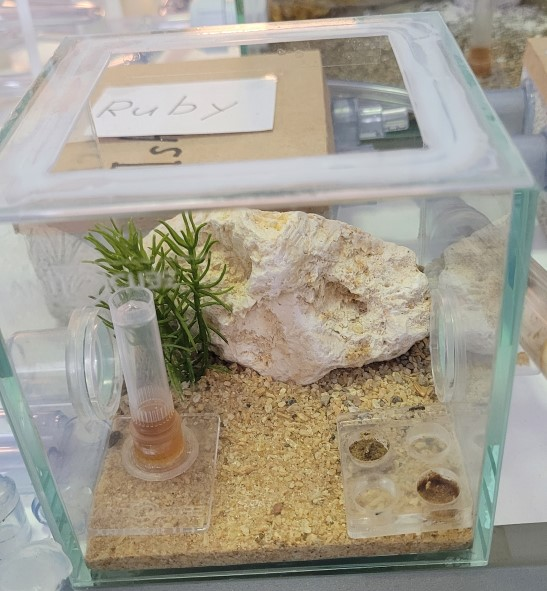
\includegraphics[width=.8\linewidth]{resources/F-rufibarbis.jpg}
    \caption[Waldameisen]{Waldameisen}
  \end{minipage}%
  \begin{minipage}{.5\textwidth}
  \end{minipage}
\end{figure}

\section{notwendig 2--3x die Woche}

\subsection{Zucker}\label{sec:Ameisen_sub:Zucker}

\begin{wrapfigure}{R}{0.3\textwidth}
  \centering
  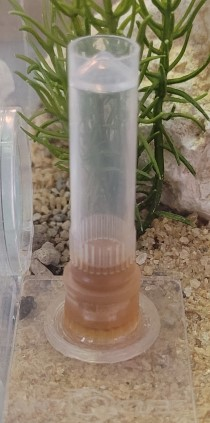
\includegraphics[width=.95\linewidth]{resources/Zucker-Fuellstand.jpg}
\end{wrapfigure}

Zucker ist überlebensnotwendig für die erwachsenen Tiere, sonst haben sie nicht die Energie,
um in der Arena nach Futter zu suchen und die gesamte Kolonie kann sterben.

Daher bitte bei jeden Besuch überprüfen, ob die Zuckertränken noch voll sind oder sich Schimmel bildet.
Fällt der Füllstand in den geriffelten Bereich der Röhrchen wie im Bild rechts zu sehen,
muss es mit einem frischen ersetzt werden.
Die leere Tränke mit der Pinzette aus der Arena heben und etwaige Ameisen mit dem Pinsel abstreifen.
Bereits befüllte Röhrchen liegen im Kühlschrank, einfach in eine frische Basis stecken (stehen auf dem Tisch)
und in die Arena stellen.
Sollten die ausgehen und ein frisches befüllt werden müssen, dann einfach vorsichtig mit Honig aus der Quetschtube auffüllen
(geht gerade so rein, wenn man vorsichtig ist und gut zielt\ldots{}).

Sollten große Reagenzgläser mit Zuckerwasser angeschlossen sein, besteht keine Gefahr,
dass sie leergetrunken werden, jedoch setzen diese sehr schnell Schimmel an.
Ist das der Fall, bitte wie oben beschrieben eine Tränke in die Arena stellen und
wenn möglich das verschimmelte Reagenzglas entfernen.
Entleeren wäre in dem Fall auch super, dazu den Wattestopfen mit der geraden Pinzette herausziehen.

\subsection{Wasser}\label{sec:Ameisen_sub:Wasser}
Ameisen brauchen Zugang zu sauberem Wasser, daher bitte regelmäßig alle Wasserröhrchen\todo{Bild von Wasserröhrchen}
(üblicherweise eines pro Kolonie) kontrollieren:

\begin{itemize}
  \item\textit{Leichte Verfärbung des Wassers} \\
  kein Problem für 1--2 Wochen, wechseln kann warten bis ich zurück bin
  \item\textit{Starke Verfärbung des Wassers} \\
  wenn möglich bitte wechseln\todo{Prozess beschreiben}
  \item\textit{deutlicher Schimmel auf der Watte} \\
  bitte umgehend wechseln\todo{Prozess beschreiben}
  \item\textit{Erde auf der Watte} \\
  das ist normales Verhalten der Ameisen, kein Eingriff nötig
  \item\textit{Ameisenbrut im Reagenzglas} \\
  sollte das Nest zu trocken werden, entscheiden die Ameisen oft, ihre Brut in das Wasserglas zu verlegen.
  In diesem Fall natürlich nicht entfernen, selbst wenn sich Schimmel bildet.
  Einfach das Nest extra befeuchten und beim nächsten Besuch beobachten.
\end{itemize}

Tritt nichts davon auf, reichen die Röhrchen wochenlang, im Gut-Fall muss also gar nicht gewechselt werden.

\section{notwendig 1x die Woche}

\subsection{Nest befeuchten}\label{sec:Ameisen_sub:Befeuchten}
Die Nester der Wegameisen (mit der roten Folie) halten ihre Feuchtigkeit bis zu meiner Rückkehr,
nur das Nest der Waldameisen aus Luftbeton (mit der Abdeckung aus Pappe darauf) muss regelmäßig befeuchtet werden:
\begin{enumerate}
  \item Spritze mit stillem Mineralwasser füllen\todo{Bild on Spritze und Wasserflasche}
        (Leitungswasser kann Chlor enthalten, kann im Notfall aber auch verwendet werden)
  \item Papp-Deckel vorsichtig abnehmen (um die Bewohner nicht zu stören).\\
        Nicht erschrecken: darunter ist eine Glasscheibe, durch welche die Ameisen beobachtet werden können, aber sie können nicht heraus!
  \item Spritze in das Loch in der Scheibe einführen und langsam entleeren, bis Wasser aus dem Loch herauskommt.
  \item Spritze entfernen und ggf. überstehendes Wasser damit wieder aufsaugen
  \item Pappdeckel wieder aufsetzen
\end{enumerate}
Dieser Prozess darf gerne einmal zu Beginn des Besuchs durchgeführt und dann am Ende nochmal wiederholt werden,
wenn etwas Wasser in den Stein eingezogen und wieder Platz im Reservoir ist.

\subsection{Füttern}\label{sec:Ameisen_sub:Fuettern}
Ameisen brauchen Protein zum Wachsen, vor allem im Larvenstadium.
Erwachsene Ameisen brauchen kein Protein mehr, werden aber ihre Aktivität in der Arena
(und Ausbruchsversuche) verstärken, wenn nicht genug Protein da ist um die Jungen zu füttern.
Sollte mehrere Tage kein Protein zur Verfügung stehen, fangen Teile der Brut an zu sterben.
Ein paar Tage zu spät zu füttern stellt aber kein Problem dar, Ameisen legen Vorräte an.

\begin{itemize}
  \item Jede der Wegameisen Kolonien bekommt eine große Schabe
        oder zwei bis drei Heimchen/Heuschrecken.
  \item Die Waldameisen bekommen eine kleine bis mittelgroße Schabe oder ein Heimchen.
        Diese Schalen sind dazu zu verwenden:\todo{Bild von Schalen hinzufügen}
\end{itemize}

\subsubsection{Lebendfutter präparieren}
Schaben, Heimchen etc.\ müssen vor der Fütterung getötet werden,
das verhindert Verletzungen der Ameisen und das Leiden der Futtertiere.
Hierfür steht die grüne Schneidmatte als Unterlage zur Verfügung.
Das Futtertier mit Pinzette über die Futterschale halten und mit der blauen Bastelschere den Kopf abschneiden.
Bei Schaben zusätzlich noch 1--2 Mal den Köper durchschneiden, sie laufen sonst auch ohne Kopf davon.

Wenn sich das Tier aus der Pinzette befreit und zu Boden fällt, einen ruhigen Kopf behalten!
Die Argentinischen Schaben rennen nicht sonderlich schnell
und auch Heimchen sind einfach wieder einzufengen, wenn man ruhig bleibt.
Ein Fangbecher steht bereit.

\subsubsection{Alternative}
Wenn Schaben oder Heimchen nicht verfügbar sind, oder der Mut fehlt, kann Instant-Futter gegeben werden:
Für die Wegameisen eines der großen runden Schälchen etwa zur Hälfte mit Insektenpulver\todo{Bild von Pulver} füllen
\todo{Bild von gefüllter Schale} und etwas Wasser einträufeln\todo{Bild von Spritze und Wasserflasche, Anzahl Tropfen angeben}.
Die Waldameisen bekommen zwei der kleinen Aussparungen im Vierertopf\todo{Bild vom gefüllten Vierertopf} auf dieselbe Weise gefüllt.
Es gibt zwei Arten von Insektenpulver im Kühlschrank, oberes Fach links, darf gerne abgewechselt werden.
Sind diese leer finden sich weitere Röhrchen in Tüten im Tiefkühlfach, ebenfalls oberes Fach.

\section{Ausgebüchste Ameisen einfangen}
Wenn Ameisen entkommen sind, keine Panik! Sie \textit{wollen} wieder zurück ins Nest und entfernen sich nicht weit,
sie können einzeln mit einem Pinsel aufgetupft und wieder in die Arena gesetzt werden.
Größere Ausbrüche auf diese weise zu bekämpfen, kann zeitraubend sein.
Hinterher nach dem Loch suchen:
\begin{itemize}
  \item Ist ein Stöpsel herausgerutscht?
  \item Hat sich ein Schlauch gelöst oder ein Reagenzglas abgegangen?
  \item Ist eine der Schlauchkreuzungen aufgegangen? (Der Heißkleber hat sich ggf.\ abgelöst)
  \item Quetschen sie sich durch einen Spalt zwischen Arena und Deckel?
  \item Ist die weiße Barriere am Deckel an einer Stelle unterbrochen?
        (Hierfür muss man die Ameisen eine Weile bebachten um zu sehen, wo sie über die Barriere treten)
\end{itemize}

  \chapter{Argentinische Schaben (Dubia Roaches)}

\section{Säubern}
Gute Nachricht, das ist nicht nötig!

\section{Füttern}

\subsection{Trockenfutter}
Trockenfutter ist leicht anzubieten da es nicht schimmelt, einfach 1--2 Mal die Woche kontrollieren
und bei Bedarf die Futterschale auffüllen.
Trockenes Katzenfutter befindet sich im Gemüsefach des Kühlschranks, Haferflocken auf dem Tisch.
Nach Belieben entweder mischen oder einfach abwechseln.

\subsection{Frischfutter}
Gesund ernährte Schaben sind auch selbst gesünderes Futter, optional kann also gerne alle paar Tage
frisches Gemüse/Obst/Früchte gegeben werden. Sie freuen sich auch über Küchenreste.
Vorgeschnittenes Futter (Äpfel, Karotten, Pfirsich) liegt im oberen Fach des Tiefkühlers,
idealerwiese etwas antauen lassen bevor es den Schaben angeboten wird.

Von der Menge her nur so viel geben wie verzehrt wird, bevor es Schimmel ansetzt,
also z.B. 3--4 Karottenscheiben, ein Apfel-/Pfirsichstück oder ähnliches.
Lieber zu wenig geben als Schimmel riskieren.
Beim nächsten Besuch bitte kontrollieren und Reste entsorgen.

\section{Wasser}
Schaben ertrinken leicht, daher steht das Wasser in Form von Wasserperlen zur Verfügung.
Diese sollten nicht für mehr als einen Tag völlig austrocknen
(eine volle Schale Wasserperlen hält allerdings locker mehr als eine Woche),
daher lieber früher als später frische Perlen ansetzen:
\begin{enumerate}
  \item einen halben Teelöffel frische Perlen in Schale geben
  \item bis etwas über die Hälfte mit stillem Mineralwasser füllen
  \item abgedeckt einige Stunden (ggf. über Nacht) aufquellen lassen
  \item die ausgetrockneten Perlen in den bereitstehenden Becher umleeren
  \item frisch aufgequollene Perlen vorsichtig in die Wasserschale umfüllen\\
        (die Dinger springen wild umher)
\end{enumerate}
\begin{figure}[H]
  \begin{minipage}{.5\textwidth}
    \centering
    
\includegraphics[width=.8\linewidth]{resources/Wasserperlen.jpg}
  \end{minipage}%
  \begin{minipage}{.5\textwidth}
    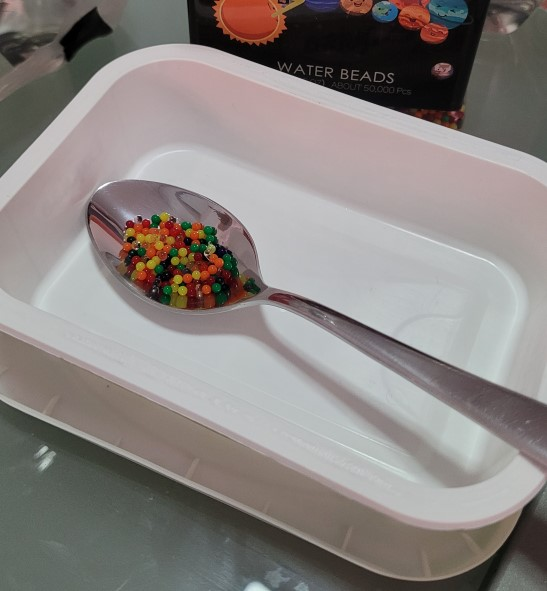
\includegraphics[width=.8\linewidth]{resources/Wasserperlen-abmessen.jpg}
  \end{minipage}
  \caption[Wasserperlen]{Menge an zu verwendender Perlen}
\end{figure}

\end{spacing}

\clearpage

\pagestyle{plain}


% Literaturverzeichniss - Ab hier wieder Roemische Seitenzahlen

\pagenumbering{roman}
\ifbibliography{}
  \setcounter{page}{\theromanPagenumber}
  %\bibliographystyle{apalike}
  %\bibliography{literatur}
  \printbibliography[title=\prefbiblioname]
  \onehalfspacing{}
  \clearpage
\fi

\pagestyle{empty}
\thispagestyle{empty}

\end{document}
% chktex 17 ignore deliberately unmatched numnber of parentheses (there's a single ')' in the preamble)
